\newpage
\begin{center}
\textbf{ГЛАВА 3}\\
\textbf{ДИССИПАТИВНЫЕ ФАЗОВЫЕ ПЕРЕХОДЫ В ПЫЛЕВОЙ (КОМПЛЕКСНОЙ) ПЛАЗМЕ}
\end{center}
\refstepcounter{chapter}


% \section*{}
\addcontentsline{toc}{chapter}{ГЛАВА 2. Диссипативные фазовые переходы в пылевой (комплексной) плазме}
%\section{Расчет спектров в МД}

\section{Фазовые диаграммы в диссипативных системах}

В диссипативных системах важную роль играет нелинейная динамика ~\cite{Lichtenberg}, которая проявляется в таких системак как: нелинейные осцилляторы, квази-регулярное движение, странные аттракторы и хаос \cite{physrep.2005, Rabinovich2006, Ernest2015}.

Невзаимность сил может играть ключевую роль в динамике активной материи ~\cite{Vicsek2012} или таких многоагенных систем, как: крабы ~\cite{Yukio2018}, насекомые ~\cite{Sumpter2006}, косяки рыб ~\cite{Katz2013}, стаи животных ~\cite{Francesco2015} или животные клетки ~\cite{Copenhagen2018}. На сегодняшний день данные системы привлекают к себе наибольший интерес с точки зрения межчастичных взаимодействий в диссипативных многочастичных систем. Не смотря на это, до сих пор плохо изучен вопрос того, как изменения в силе внутричастичных взаимодействиях влияют на динамику таких систем. 

Известно, что в коллоидных суспензиях и пылевой плазме эффективные взаимодействия могут быть невзаимными, так как они помещены в неравновесную среду ~\cite{Royall2015, 10.1103/PhysRevX.5.011035}. Примерами таких сред могут быть: оптические лучи, потоки ~\cite{PhysRevLett.91.248301,Hayashi2006, Sriram2012, Carlos2011}, диффузиофорез ~\cite{PhysRevLett.105.218103, Hassan2017, Huan2016} и 
плазменные вейки ~\cite{10.1070/pu1997v040n01abeh000201, 10.1103/physreve.64.046403, 10.1039/c0sm00813c, 10.1103/physreve.54.4155, 10.1103/physreve.53.2757, 10.1103/physreve.93.063201, 10.1209/0295-5075/111/50003, 10.1063/1.4953225}. 


Взаимодействия, вызванные потоками плазмы, являются невзаимными, что приводит к резким и фундаментальным изменениям в динамике внутри диссипативных систем. Эти изменения регулируются выделением энергии и диссипацией \cite{10.1039/c8sm01836g} и могут привести к многотемпературным стационарным состояниям\cite{10.1103/physrevx.5.011035}, одно- и двухступенчатой термической 
активации \cite{10.1103/physreve.96.043201, 10.1103/physreve.100.023203, 10.3367/ufne.2019.01.038520}, термоакустической неустойчивости \cite{10.1103/physrevlett.121.075003} или бистабильности \cite{10.1103/physrevlett.119.178004}. 
% Данные выводы раскрывают физические принципы, управляющие коллективным поведением диссипативных систем.

В качестве модельной системы, способной к плавлению и термической активации, обычно рассматривают монослой заряженных микрочастиц в потоке плазмы. Рассмотрим, например, частицы, взаимодействующие посредством отталкивающего потенциала Юкавы (Дебая-Хукеля), где нересепрокальность обеспечивается за счет плазменных вейков, образующихся под каждой частицей. Частицы помещают в параболическую потенциальную яму и моделируют в термостате Ланжевена []. 
Устойчивые состояния состояния получают с помощью моделирования MD (Molecular Dynamic Simulation) и с использованием балансового подхода ~\cite{10.1039/c8sm01836g}. 

Если взять конкретные модель взаимодельствия и плотность системы, то ее динамика определяется временем затухания $\tau$, частотой конфайнмента $\Omega$ и температурой термостата $T_{th}/T_m$, которая нормируется на температуру плавления $T_m$ соответствующего двумерного кристалла Юкавы).

\begin{figure}[htbp]
\centerline{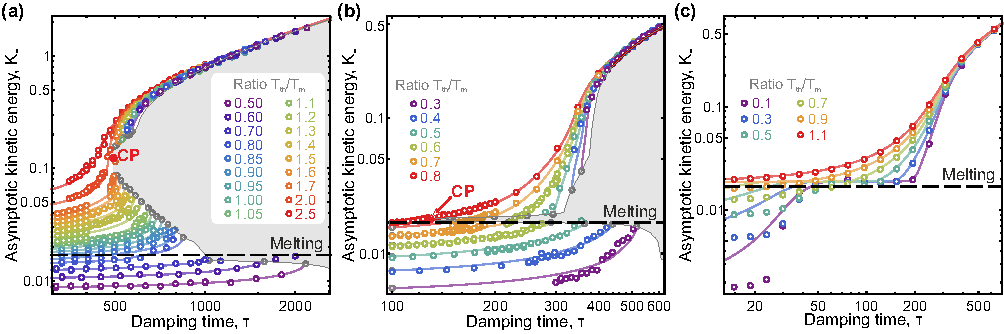
\includegraphics[width=1.0\linewidth]{Ris/DPD-Figure1.pdf}}
\caption{Диссипативные фазовые диаграммы при различных значениях конфайнмента $\Omega$}
\label{DPD-Figure1}
\end{figure}


При сильных значениях конфайнмента система показывает диссипативный спинодальный распад между неактивированным и активированным состояниями и имеет  диссипативную критическую точку (СР), показанную на рис. \ref{DPD-Figure1}(а). В зависимости от 
энергии $K_{\infty} / T_m \lessgtr 3/2$, система может существовать в жидком или твердом состояниях, 
а линии с одинаковыми значениями температуры плавления $T_{th}$ играют роль изотерм. Диссипативный 
спинодальный распад возможен только в том случае, если $T_{th}$ меньше критической температуры термостата. Так как критическая точка находится выше линии плавления в 
энергии $K_{\infty}$, жидкость может существовать в неактивированных или активированных состояниях при $0.8 \leq T_{th}/T_m \leq 1.6$.


При уменьшении силы конфайнмента критическая точка смещается вниз к линии плавления, как показано на рис.\ref{DPD-Figure1}(b). 
В данном случае значения энергии $K_{\infty}$ в критической точке и при плавлении практически совпадают, и неактивированное жидкое состояние становится неустойчивым. 
При дальнейшем уменьшении величины конфайнмента $\Omega$ фазовая диаграмма резко меняется, как показано на рис.\ref{DPD-Figure1}(c). Для $\Omega^2 = 9$ средняя энергия $K_{\infty}(\tau)$ вблизи линии плавления превращается 
в вертикальную линию при $ T_{th}/T_m \leq 0.6$, что говорит о значительных изменениях в динамике системы между $\Omega^2 = 9.75$ и $\Omega^2 = 9$. В связи с этим изучение влияния силы конфайнмента 
на вид спектра элементарных возбуждений и мощности энерговыделения является важной и актуальной проблемой.

Диссипативные фазовые диаграммы показаны на рис \ref{DPD-Figure1},
где асимптотические значения средней кинетической энергии
на одну частицу $K_{\infty}$ были получены при различных $\tau$, $T_{th}/T_m$,
и различных значениях конфайнмента ($\Omega = 11.25, ~9.75,~ 9.0$).
Пунктирные черные линии соответствуют линии плавления $K_{\infty} / T_m = 3/2$, где $K$ в данном случае играет роль, аналогичную  температуре. 
Серые зоны , полученные с помощью балансового подхода, являются областями диссипативного спинодального распада, в которых система термически неустойчива. Важно, что результаты, полученные моделированием MD, хорошо согласуются с балансовым подходом (сплошная линия). Расхождения наблюдаются только на низких значениях $K_{\infty}$ и $\tau$ и обусловлены особенностями энергии
высвобождение при нестабильности связи мод \cite{10.1103/physreve.63.016409, 10.1103/physrevlett.104.195001}.

\section{Высвобождение энергии}

Устойчивое состояние диссипативной системы определяется балансом между энергиями выделения и диссипации \cite{10.1039/c8sm01836g}, который в данном случае обеспечивается невзаимностью взаимодействия и демпфированием.
Диссипация контролируется скоростью затухания и температурой термостата, а величина конфайнмента влияет на возбуждения в системе внутри плоскости и перпендикулярно ей, таким образом влияя на мощность энерговыделения. 

% Чтобы разобраться в механизмах
% ответственный за поведение, показанное на рис. 1, мы рассчитали
% зависимости мощности энерговыделения $P_{NR} (K)$
% как функция энергии $K$ вместе с возбуждением спектры кристаллов и жидкостей [] при различных $\Omega^2$.
\begin{figure}[htbp]
\centerline{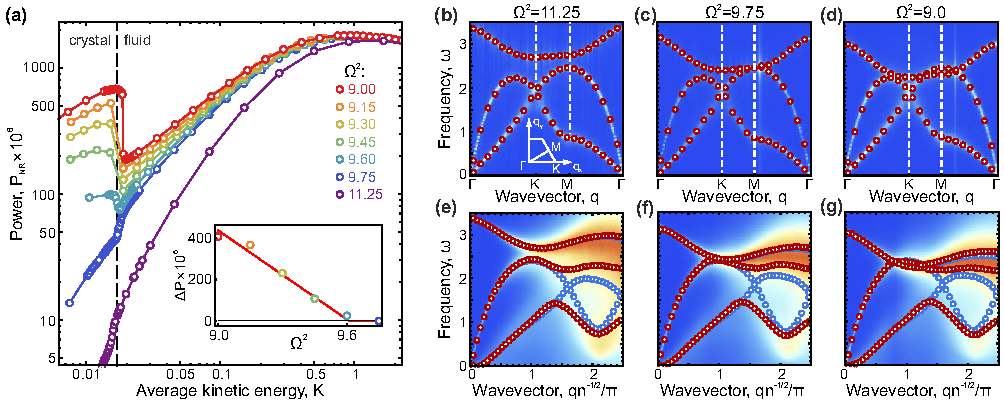
\includegraphics[width=1.0\linewidth]{Ris/DPD-Figure2.pdf}}
\caption{Мощность энергии высвобождения и спектры возбуждения при различных значениях конфайнмента}
\label{DPD-Figure2}
\end{figure}

Мощность высвобождения энергии при различных значениях конфайнмента $\Omega^2$ показана на рис.\ref{DPD-Figure2}(а), где пунктирная черная линия показывает, где находится линия плавления. На рис.\ref{DPD-Figure2}(а) 
так же можно видеть зазор $\Delta P$ между мощностью высвобождения энергии в кристалле и жидкости на линии плавления. В кристалле $\Delta P = 0$, энергия не высвобождается при $\Omega^2 > \Omega^2_{*} \approx 9.5$, и $P_{NR}$ монотонно зависит от $K$. Величина $\Delta P$ становится положительной в $\Omega^2 \leq \Omega^2_{*}$ и 
растет приблизительно линейно, как показано сплошной красной линией на вставке на рис.\ref{DPD-Figure2}(а).

В этом диапазоне значений $\Omega^2$ высвобождение энергии в кристалле становится значительно больше, чем в жидкости, и стабильно растет
при $\Omega^2 \rightarrow 9.0$, что приводит к $\Delta P > 0$. Это означает, что при одних и тех же условиях кристалл термически активируется, а жидкость -- нет. 



При $\Omega^2 \approx \Omega^2_{*}$ энергии высвобождения в кристалле и жидкости становятся
равными возле линии плавления. 
Данное поведение можно более делально изучить с помощью дисперсионных соотношений $\omega(q)$ в кристаллах и жидкостях, которые изображены на рис.\ref{DPD-Figure2}(b-g).
При сильном значении конфайнмента продольные (оптические) ветви, лежащие вне плоскости, и акустические ветви, лежащие внутри плоскости, не пересекаются, как это видно на рис.\ref{DPD-Figure2}(b),(e). 
Однако, по мере приближения $\Omega^2$ к $\Omega^2_{*}$ ветви сближаются друг к другу и затем
пересекаются при $\Omega^2 \approx \Omega^2_{*}$, способствуя сильному выделению энергии за счет их взаимодействия, что, как правило, характерно для невзаимных систем \cite{10.1103/physreve.63.016409, 10.1103/physrevlett.104.195001, 10.1103/PhysRevLett.113.135002, 10.3367/ufne.2019.01.038520}, как показано на рис.2(c,d) и (f,g). 


Спектры показаны на рис.\ref{DPD-Figure2}(c-g) синими и красными символам. Результаты, полученные различными подходами, хорошо согласуются друг с другом
в кристалле и при малом $q$. При $qn^{-1/2} / \pi \geq 1.5$ продольные и поперечные моды в жидкости пересекаются и становятся гибридизированными. 

Таким образом, рост $\Delta P$ в мощности энерговыделения коррелирует с
пересечением оптических и продольных акустических мод в жидкости, которое отвечает за
принципиальное изменение диссипативной фазовой диаграммы показано на рис. \ref{DPD-Figure2}(b, c) при $\Omega^2 = \Omega^2_{*}$. 
На самом деле, зазор $\Delta P$ в мощности $P_{NR}(K)$, как результат плавления, приводит к  динамическому поведению системы (в динамике средней кинетической энергии $K$), которое называется странным аттрактором.



\section{Странный аттрактор}

Увеличение разности $\Delta P$ в мощности энергии высвобождения приводит к колебанию энергии $K(t)$  вокруг плато, наблюдаемого на рис.\ref{DPD-Figure1}(c), что соответствует динамике странных аттракторов, которые
,в свою очередь вызваны интерференцией активации и плавления. Данное поведение проиллюстрировано на рис.\ref{DPD-Figure3}, где на панели (а) изображены те же данные для $K_{\infty}$ при $T_{th} = T_m = 0.1$, что и на
рис.\ref{DPD-Figure1}(c), при которых плато находится в диапазоне $40 \lesssim \tau \lesssim 200$.

Как видно на рис.\ref{DPD-Figure3}(b), при малых и больших значениях $\tau$, $P_{NR}(K)$ и $P_{d}(K)$ пересекаются в одной точке, которая соответствует устойчивому состоянию. Однако, при значении $\tau = 97$, которое соответствует 
выходу зависимости на плато (см. рис. ), система должна была находиться в устойчивом состоянии, в зазоре, как показано на рис. , 
%Зависимости мощности энерговыделения $P_{NR}(K)$ и диссипации $P_[D}(K)$ (при различных значениях) показаны на рис.\ref{DPD-Figure3}(b). Мы рассмотрели три репрезентативных значения = 30, 97 и 246, 
%соответствующие линии и точки окрашены соответственно синим, красным и зеленым цветами на рис.\ref{DPD-Figure3}. 

При этом и кристалл, и жидкость становятся термически неустойчивыми: кристалл нагревается и стремится расплавиться, а жидкость охлаждается и стремиться застынуть.
Значения $K(t)$ испытывают колебания при $\tau = 97$, как показано на рис.\ref{DPD-Figure3}(с), в то время как при $\tau = 30$ и $247$ такого не наблюдается. 

Проанализировать показанную динамику системы можно так же с помощью спектральной плотности мощности (Power Spectrum Density), которая описывает мощность как функцию, деленную на 
единицу частоты (см. рис. \ref{DPD-Figure3}(d-f)). Для вычислений мощности использовалось следующее выражение: 

$PSD(\omega) = \int R(t') \exp(-i \omega t') dt'$, где $R(t') = \langle K(t)~K(t + t') \rangle / \langle К(t)^2 \rangle$,
$\langle \dots \rangle$ обозначает усреднение по ансамблю, а значение $K(t)$, соответствующее промежутку релаксации, отбрасывались.

Видно, что спектральные плотности одинаковы на малых и больших расстояниях, что демонстрирует наличие только тепловых колебаний и медленную релаксацию,
в то время как при $\tau = 97$ наблюдается широкий пик вокруг $\omega \approx 1.35  \cdot 10^{-2}$.


\begin{figure}[htbp]
    \centerline{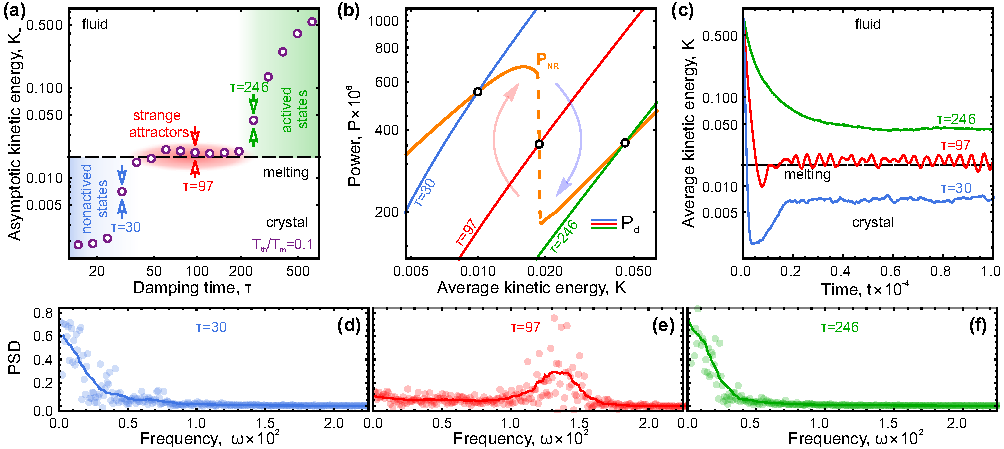
\includegraphics[width=0.95\linewidth]{Ris/DPD-Figure3.pdf}}
    \caption{Динамика странного аттрактора}
    \label{DPD-Figure3}
\end{figure}

Как известно, хаотическая динамика может быть визуализирована с помощью зависимостей, типичных для анализа нелинейных систем \cite{Lichtenberg}, 
которые показаны на рис.\ref{DPD-Figure3} в координатах $\{ K, \dot{K}, \dot{H}\}$. 
При этом система эволюционирует, демонстрируя сильные апериодические колебания и хаотические скачки 
между кристаллическим и жидким состояниями, что называется странным аттрактором. 

Наблюдаемое хаотическое поведение может быть объяснено с помощью дискретно-временной модели \cite{Lichtenberg}, предполагающая выполнение следующих соотношений:
\begin{align} \label{StAttr}
    &K_{n+1} = f(K_n), \\
    &f(K_n) = K + \eta (P_{NR}(K) - P_{d}(K)),
\end{align}

где $K_n$ - кинетическая энергия в дискретный момент времени $t_n$, $f(K)$ - функция отображения 
а $\eta$ -- параметр модели, характеризующий время инерции системы. 


Диаграмма каскада бифуркации удвоения периода для мощностей 
$P_{NR}(K)$, $P_{d}(K)$, показанных на рис.\ref{DPD-Figure3}(b) (при $\tau = 97$), изображена в цветовом формате для различных вероятностей от синего, что соответствует низкому значению, до красного, что соответствует высокому значению.
Пример функции $f (K)$ при $\eta = 1.5$ показан во вставке рис. \ref{DPD-Figure3} сплошной красной линией.

  Классический сценарий перехода к хаосу через каскады бифуркаций удвоения периодов \cite{Lichtenberg} хорошо виден на рис.\ref{DPD-Figure3}. Это обусловлено формой 
  функции $f (K)$, которая необратима и, следовательно, может привести к хаотическому поведению с образованием странных аттракторов. 
Рассматриваемая модельная система может демонстрировать при определенных условиях хаотические скачки между 
  различными состояниями, спонтанное плавление и замерзание. 
   
Можно провести оценку $\eta \approx 11$, соответствующую странному аттрактору на рис.\ref{DPD-Figure3} при $\tau = 97$, сравнивая величины 
   флуктуаций кинетической энергии на рис.\ref{DPD-Figure3}(с). Малость отношения $\eta / \tau \approx 0.11$, которая означает, что шаг дискретизации, используемый в данной модели, существенно меньше 
   характерного времени релаксации системы, оправдывает пригодность модели (1) для качественного анализа нелинейной 
   динамики в данной системе.
   
\section{Выводы}     
В данной главе были описаны диссипативные фазовые переходы в пылевой (комплексной) плазме. Был проведен анализ факторов, влияющих на устойчивость состояние диссипативной системы, было показано, что она определяется балансом между энергиями выделения и диссипации. Было обнаружено, что в результате плавления структурные корреляции на дальних расстояниях
исчезают, и
спектры флуктуаций изменяются скачкообразно, что играет решающую роль в поведении динамики системы. Было показано, что изменения структуры и вида спектров элементарных возбуждений приводят к образованию зазора в мощности энергии высвобождения между
значениями в кристалле и жидкости на линии плавления. 
При попадании мощности диссипации в зазор активированный кристалл
нагревается и имеет тенденцию плавиться, тогда как неактивированная
жидкость охлаждается и имеет тенденцию замерзать, что приводит к появлению странного аттрактора. Таким образом, данные заключения позволили связать динамическое поведение странного аттрактора
с взаимодействиями между отдельными частицами.
И диссипативные фазовые диаграммы в таких
системы могут быть легко рассчитаны с высокой точностью с помощью простого балансового
подхода.